\documentclass[a4paper,11pt]{article}
\usepackage[T1]{fontenc}
\usepackage[utf8]{inputenc}
\usepackage{lmodern}
\usepackage{hyperref}
\usepackage{caption}
\usepackage{graphicx}

\title{Cloud Computing Assignment: MPI on the cloud}
\author{Léo Unbekandt}

\begin{document}

\maketitle
\tableofcontents

\section{Settings}
\subsection{Parameters}

The experiments have been done with the following values:

Size of the square matrix: 128, 256, 512, 1024.
Number of nodes: 1, 2, 4, 8, 16 (except with 2 and 3 vCPUS VMs). This number
is limited by the quota in vCPUs (32) or Memory (50GB) and finally the
different flavors of virtual machines which have been used:
\begin{itemize}
  \item 1 - m1.tiny (512MB RAM, 1vCPU)
  \item 2 - m1.small (2GB RAM, 1vCPU)
  \item 3 - m1.medium (4GB RAM, 2vCPUs)
  \item 4 - m1.large (8GB RAM, 4vCPUS)
\end{itemize}

When a virtual machine has more than 1 vCPU, the MPI flag -npernode is used, in order
to execute one instance of the application per vCPU, otherwise. Otherwise, it is
useless to choose high quality flavors.

\subsection{Automation of the exectution}

These tests have been run using only one command to avoid a maximum of human
interactions. A ruby script has been developed to create the nodes cluster and to
destroy it. When the cluster has been built, it automatically runs ansible in
order to configure the nodes and install Open MPI on them.

Once the platform is ready, another script is able to run the experiments with
the different kinds of matrix et get the output result back. (run\_matrix\_multiply.sh)

Finally a last script (run\_experiment.sh) takes care to:
\begin{enumerate}
  \item Build a cluster with N nodes and flavor F
  \item Run MPI experiments
  \item Get the results
  \item Shutdown the cluster
  \item Restart with other parameters
\end{enumerate}

This last program takes care of everything, nothing else has to be done, except
reading and interpreting the results!

\section{Results}

The results in this section come from VMs of flavor 1, which have only one CPU.

\subsection{Small matrices computation}

The raw data results can be read in Appendix~\ref{app:rawresults}. First, for the
small matrices (128 rows/columns), it is observable that the communication between the
nodes becomes too heavy and even if the computation time is reduced, the overall
duration increased hugely. Whatever is the flavor, the performance increases
when the number of nodes is low, and then, they get strongly worse.

\begin{center}
  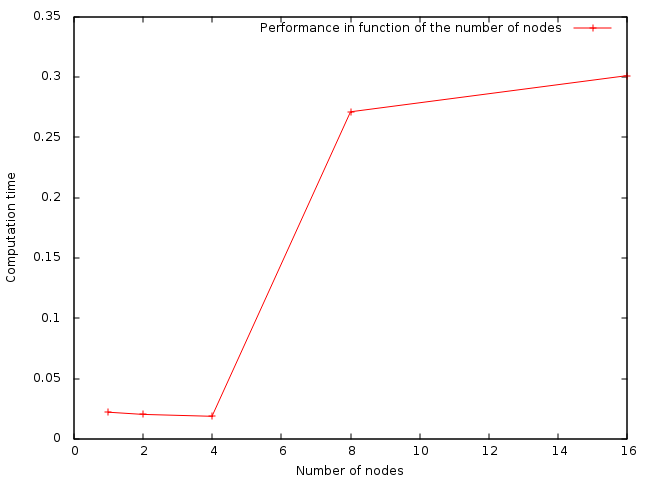
\includegraphics[width=0.8\textwidth]{./128perf.png}
\end{center}

\subsection{Large matrices computation}

In the case of large matrices computation, the results are closer to what
has to be expected, they are better and better but with a speed-up which is
not linear.

\begin{center}
  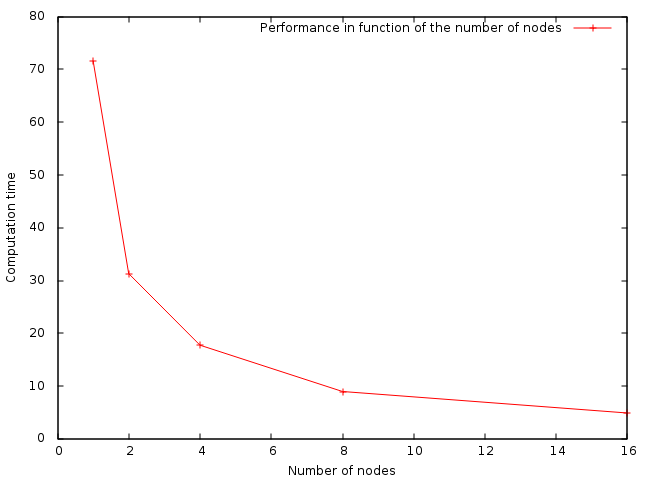
\includegraphics[width=0.8\textwidth]{./1024perf.png}
\end{center}

\subsection{Speedup Evolution}

The two previous results can be illustrated in the following graph.

\begin{center}
  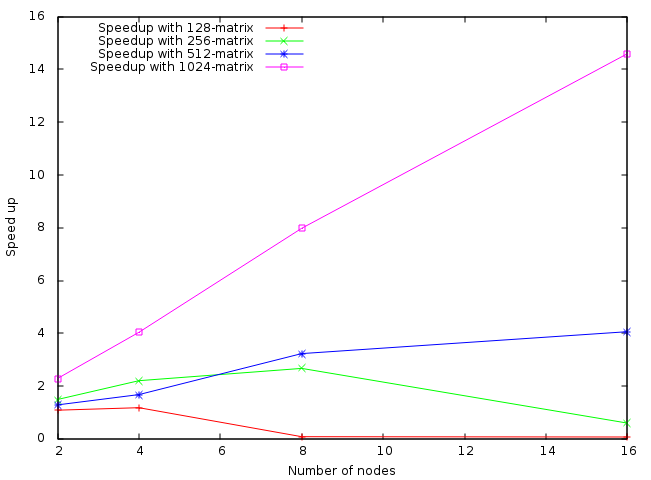
\includegraphics[width=\textwidth]{./speedup.png}
\end{center}

With a small matrix, the speed up is getting lower than 1 quickly. It means
that the execution time is increasing when the number of nodse is increasing.
However, when the matrix get bigger, the speed up increases when the number
of VMs increases.

\subsection{Cloud irregularity}

We have to keep in mind that the hardware is shared among all the user, our
tasks don't get dedicated CPUs for example. Consequently, some results may be
inadequate. For instance we can se in the measure done with flavor 3 instances,
it has been faster to compute the multiplication of a 1360x1360 matrix than a
1024x1024 matrix which is logically abnormal.

\section{Pricing}

The price for a single instance with one CPU on Amazon EC2 depends of the flavor:

\begin{itemize}
 \item m1.tiny \$0.065 per hour
 \item m1.small \$0.130 per hour
 \item m1.medium \$0.260 per hour
 \item m1.large \$0.520 per hour
\end{itemize}

For small-scale experiments like this one, the price would be completely
negligible, however for MPI operations, the lesser the communications, the
faster the execution. As a result, it is more interesting to take high-CPUs
instances. For instance, in the case of intensive computational MPI tasks, one 
m1.large is more interesting than four m1.tiny. The price per CPU is identical.

\section*{Conclusion}

To conclude. we can see that MPI on the cloud is working well, however the
communication overhead is more important than on a supercomputer and it's
important to be aware of it. Furthermore the performance may be unstable, the
instances may share their CPUs with other resource-consuming instances.



\section*{Appendices}
\appendix 
\section{Results}
\label{app:rawresults}

\begin{center}
\begin{tabular}{c | c | c | c | c}
   & 128 & 256 & 512 & 1024 \\
1  & 0.0221 & 0.1784 & 1.6523 & 43.8849 \\
2  & 0.0186 & 0.1260 & 0.9865 & 29.6860 \\
4  & 0.2568 & 0.1083 & 0.8879 & 16.5539 \\ 
8  & 0.2630 & 0.0826 & 0.5524 & 11.1385 \\
16 & 0.5145 & 0.2203 & 1.1342 & 11.8693 \\
\end{tabular}
\captionof{table}{Computation time according to the number of nodes to the size of the matrix for VMs flavor 1}
\vspace{1em}
\end{center}

\begin{center}
\begin{tabular}{c | c | c | c | c}
   & 128 & 256 & 512 & 1024 \\
1  & 0.0221 & 0.1787 & 1.6726 & 71.6537 \\
2  & 0.0203 & 0.1198 & 1.2978 & 31.3095 \\
4  & 0.0187 & 0.0811 & 0.9964 & 17.7449 \\
8  & 0.2711 & 0.0669 & 0.5174 & 8.9784 \\
16 & 0.3011 & 0.2976 & 0.4117 & 4.9098
\end{tabular}
\captionof{table}{Computation time according to the number of nodes to the size of the matrix for VMs flavor 2}
\vspace{1em}
\end{center}

\begin{center}
\begin{tabular}{c | c | c | c | c | c}
   & 128 & 256 & 512 & 1024 & 1360\\
1 & 0.0137 & 0.0937 & 0.8426 & 34.9952 & 21.3736 \\
2 & 0.0169 & 0.0758 & 0.6042 & 11.7280 & 11.0668 \\
4 & 0.2616 & 0.0698 & 0.4093 & 6.0268 & 6.4729 \\
8 & 0.3310 & 0.0868 & 0.4060 & 6.0640 & 6.0757
\end{tabular}
\captionof{table}{Computation time according to the number of nodes to the size of the matrix for VMs flavor 3}
\vspace{1em}
\end{center}

\begin{center}
\begin{tabular}{c | c | c | c | c}
   & 128 & 256 & 512 & 1024 \\
1 & 0.0223 & 0.1798 & 1.7618 & 41.7868 \\
2 & 0.0212 & 0.1254 & 1.8515 & 34.9107 \\ 
4 & 0.0213 & 0.1011 & 0.7157 & 18.3058 \\
\end{tabular}
\captionof{table}{Computation time according to the number of nodes to the size of the matrix for VMs flavor 4}
\vspace{1em}
\end{center}

\end{document}
